\section{Lavoro ed Energia}
%---------------------------------------------------------------------------
Il lavoro di una è la quantità di energia scambiata tra due sistemi,
quando avviene uno spostamento per mezzo di una forza. Matematicamente è
definito come l'integrale della forza lungo una curva, ovvero il percorso
lungo cui si sposta il corpo.
\begin{equation}
    \boxed{W = \int_\gamma d\vec s \cdot \vec F}
\label{eq:work&energy:work_def}
\end{equation}
Ne segue che la forza è sempre ortogonale allo spostamento, questa non
compierà lavoro sul corpo. Se pensiamo ad $\vec F$ come una risultante
delle forze otterremo che:
\begin{equation}
    W =  \int_\gamma d\vec s \cdot \sum_{k=1}^n\vec F_k =
    \sum_{k=1}^n \int_\gamma d\vec s \cdot \vec F_k = \sum_{k=1}^n W_k
\label{eq:work&energy:work_sum}
\end{equation}
Il lavoro totale può essere visto come la somma dei lavori delle singole
forze che costituiscono $\vec F$.
Se il lavoro è positivo, allora di dice lavoro motore, mentre se è negativo
si dice lavoro resistente.
Il lavoro essendo un'energia è misurato nel S.I. con il $(J)$ Joule.
Un Joule è definito come l'energia scambiata da una forza di un Newton, per
compiere uno spostamento di un metro lungo la sua stessa direzione:
$1J = 1N\cdot 1 m$. 
\subsection{Potenza}
La potenza esprime la velocità con cui viene trasferita una particolare forma
di energia. Adesso parleremo di potenza meccanica, definita come la derivata
rispetto al tempo del lavoro, ed è misurata in Watt $(W)$.
Una potenza di un Watt trasferisce un Joule in un secondo.
\begin{equation}
    \boxed{P=\frac{dW}{dt}}
\label{eq:work&energy:power_def}
\end{equation}
\subsection{Lavoro come variazione di energia cinetica}
Scriviamo il lavoro infinitesimo per una forza generica data da
$\vec F = m\vec a$.
\begin{equation}
    dW = \vec F\cdot d\vec s = ma_tds = m\dot v ds = mv dv 
\end{equation}
Integrando otterremo che il lavoro per spostare il corpo dal punto $A$ al
punto $B$ sarà:
\begin{equation}
    W = \int_{v_A}^{v_B}mvdv = \frac12mv_B^2- \frac12mv_A^2
\end{equation}
Quindi definendo l'energia cinetica, l'energia associata al movimento di un
corpo, come $K = \frac12 mv^2=\frac{p^2}{2m}$, otteniamo che:
\begin{equation}
    W = K_B - K_A = \Delta K
\label{eq:work&energy:w=dk}
\end{equation}
\subsection{Lavoro della forza gravitazionale}
Prendiamo il caso in cui la forza peso faccia spostare un corpo di massa $m$
da un punto $A$ ad un punto $B$, a quota più bassa di $A$. Supponiamo che il corpo segua un percorso a piacere, purché vada da $A$ a $B$. quindi prendo un asse verticale $z$ diretto verso l'alto, otterremo che:
\begin{figure}[htbp]
    \begin{center}
        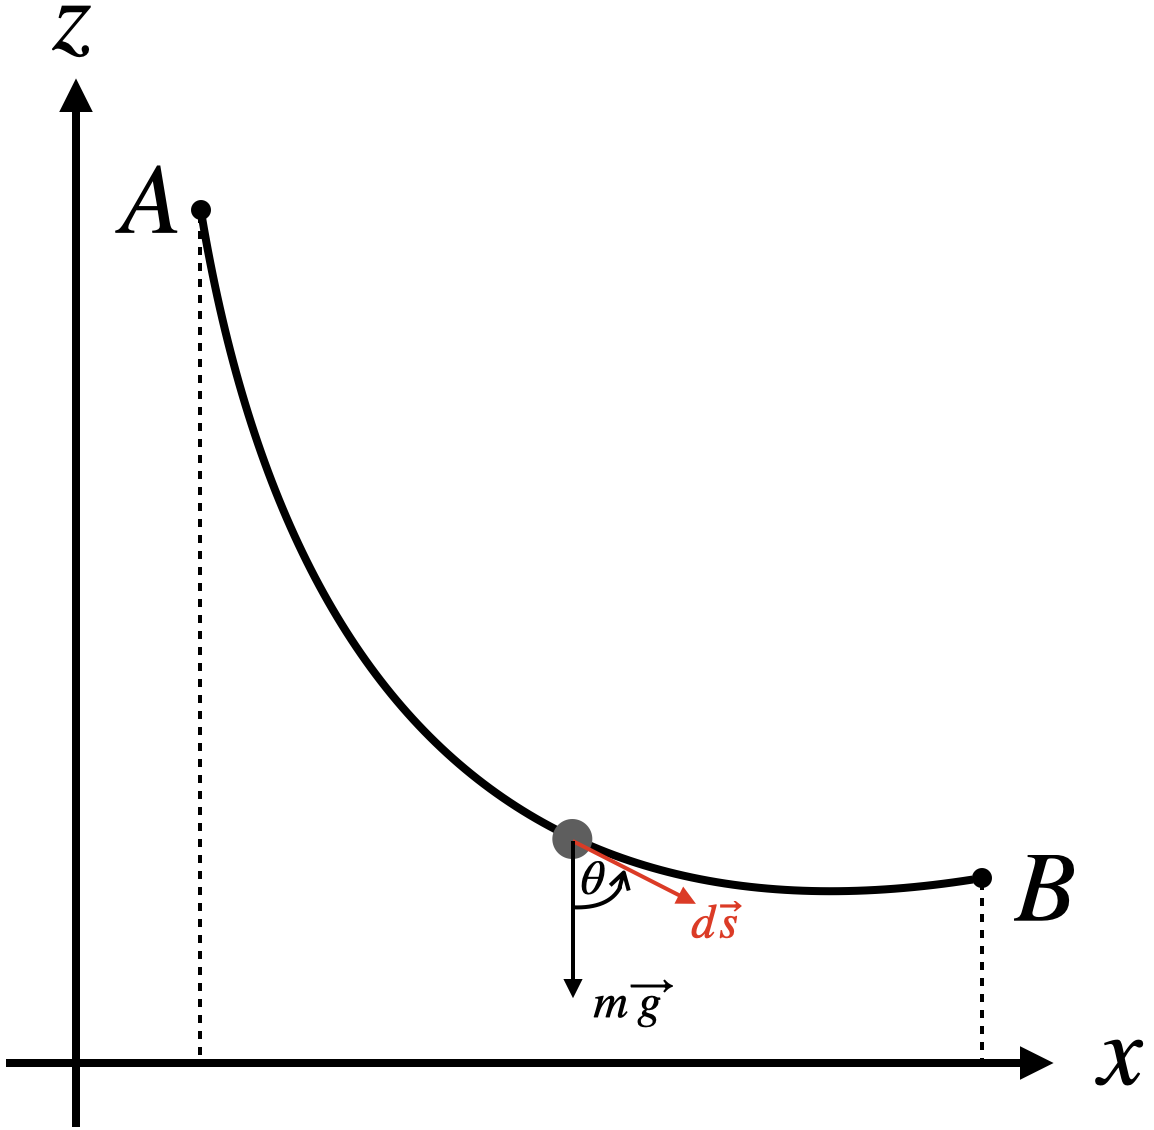
\includegraphics[width=10cm]{images/lavorog.png}
        \caption{Rappresentazione del lavoro infinitesimo lungo un tratto
        elementare di curva $d\vec s$ del forza gravitazionale
        $\vec F_p = m\vec g$.}
\end{center}
\label{fig:work&energy:P_work}
\end{figure}

\begin{equation}
    W = \int_A^Bd\vec s \cdot\vec F_p = -mg\int_A^Bds\cos\theta =
    -mg\int_A^Bdz = -mg\sx z_B-z_A\dx
\end{equation}
Ovvero definendo l'energia potenziale gravitazionale come $U = mgz$, abbiamo
che il lavoro è meno la variazione di energia potenziale:
\begin{equation}
    W = U_A-U_B = -\Delta U
\label{eq:work&energy:w=-du}
\end{equation}
imponendo uguali le equazioni (\ref{eq:work&energy:w=dk}) e (\ref{eq:work&energy:w=-du})
otteniamo il principio di conservazione dell'energia meccanica $E = K + U$.
\begin{multline}
    \Delta K = -\Delta U\seg K_B-K_A = U_A -U_B\seg
    \\\seg K_A+U_A = K_B+U_B\seg
    \boxed{E_A = E_B}
\end{multline}
\subsection{Lavoro della forza elastica}
Calcoliamo il lavoro di una forza elastica diretta lungo
$x$: $\vec F_e = -kx\hat\imath$.
\begin{equation}
    W = -k\int_A^Bdx x = \frac12 kx_A^2-\frac12 kx^2_B\quad\quad
    U_e = \frac12 kx^2\seg W = -\Delta U_e
\label{eq:work&energy:elastic_energy}
\end{equation}
\subsection{Lavoro della forza d'attrito radente}
La forza d'attrito, essendo sempre diretta in verso opposto alla velocità
produce un lavoro negativo, ovvero sempre resistente. L'integrale sulla
curva dipende dal percorso scelto, al contrario delle forze conservative,
e quindi in un percorso chiuso il lavoro d'attrito sarà diverso da zero.
\begin{equation}
    \vec F_a = -\mu_d N \hat u_v\seg W_a = -\mu_d\int_A^BdsN =
    -\mu_dN\Delta s
    \label{eq:work&energy:work_friction}
\end{equation}
\subsection{Lavoro di forze conservative e non conservative}
Come abbiamo visto, il lavoro di una forza conservativa, che ammette
un'energia potenziale, non dipende dal percorso su cui si integra, ne segue
che se scegliamo un percorso chiuso l'integrale sulla curva chiusa sarà
sempre nullo.\\
Quindi se $\vec F$ è una forza conservativa ne segue che:
\begin{equation}
    \boxed{\oint_\gamma d\vec s \cdot F = 0}
\label{eq:work&energy:conservative_force}
\end{equation}
Dunque in questi casi che l'energia meccanica si conserva, quindi l'energia
meccanica nello stato iniziale è uguale all'energia meccanica nello stato
finale:
\begin{equation}
    \boxed{E_i = E_f}
\label{eq:work&energy:Ei=Ef}
\end{equation}
Mentre nel caso in cui sono presenti forze non conservative, il lavoro delle
forze non conservative non è nullo ed è pari alla variazione di energia
meccanica. E dato che durante il processo si dissipa energia:
\begin{equation}
    \boxed{W_{NC} = \Delta E = E_f- E_i < 0}
\label{eq:work&energy:Ei>Ef}
\end{equation}
Se prendiamo una generica forza $\vec F_{\sx x,y,z\dx} = \sx F_x,F_y,F_z\dx$,
se supponiamo che essa sia conservativa possiamo scrivere che:
\begin{equation}
    \int_A^Bd\vec s\cdot \vec F = \int F_xdx+F_ydy+F_zdz
\end{equation}
Ora se ammettiamo l'esistenza di un'energia potenziale, tale per cui la forza
è il suo gradiente cambiato di segno:
\begin{equation}
    \vec F_{\sx x,y,z\dx} = -\vec\nabla U_{\sx x,y,z\dx} = -\sx\frac{\partial U}{\partial x},\frac{\partial U}{\partial y},\frac{\partial U}{\partial z}\dx
\label{eq:work&energy:gradient}
\end{equation}
Trovandoci in questa situazione avremo che:
\begin{equation}
    \int_A^B F_xdx+F_ydy+F_zdz = -\int\vec \nabla U\cdot d\vec x = -\int dU = -\sss U_{(B)}-U_{(A)}\ddd = -\Delta U
\end{equation}
Come possiamo notare i risultati ottenuti nelle equazioni (\ref{eq:work&energy:w=-du})
e (\ref{eq:work&energy:elastic_energy}),sono in realtà molto più generali e,
data una forza esprimibile come il gradiente di un'energia potenziale
(cambiato di segno), si avrà che il lavoro da un punto $A$ a un punto $B$
seguendo una qualsiasi curva, sarà pari a meno la variazione di energia
potenziale. Di conseguenza una volta appreso queso fatto, possiamo capire
facilmente il perchè dell'equazione (\ref{eq:work&energy:conservative_force}).
Se si sceglie una curva chiusa, punto $A$ coincide con il punto $B$ dunque
dato che l'energia potenziale iniziale e finale sono uguali, il lavoro è
nullo.\\
Sotto le ipotesi di forze conservative si può dimostrare facilmente l'equazione
(\ref{eq:work&energy:Ei=Ef}), ovvero la conservazione dell'energia meccanica.
\begin{equation}
    \frac{dE}{dt} = \frac12m\frac{d}{dt}v^2+\frac{dU}{dt} =
    \vec v\cdot m\frac{d\vec v}{dt} + \frac{d\vec x}{dt}\cdot\vec\nabla U =
    \vec v\sx m\vec a + \vec\nabla U\dx = 0
\label{eq:work&energy:energy_conservation}
\end{equation}